% paper template

\documentclass[10pt,reqno,final]{amsart}
%\documentclass[10pt,reqno,draft]{amsart}

% package for mathematics
\usepackage{amsmath,amssymb,amsthm}
% package for RSFS fonts in maths
\usepackage{mathrsfs}
% package for special symbols
\usepackage{pifont}
% package for multilingual support
\usepackage[english]{babel}
% package for figures
\usepackage{graphicx}
\usepackage{subfig}
% package for hyperlink
\usepackage{hyperref}
% package for layout of list
\usepackage{enumitem}
% package for showing keys in draft mode
\usepackage[notcite,notref]{showkeys}
% package for color
\usepackage{color}
% package for table
\usepackage{tabularx}
\usepackage{booktabs}
\usepackage{array}
\usepackage{makecell}
% package for multiple columns and rows
\usepackage{multirow,multicol}
% package for caption
\usepackage{caption}
% package for algorithm
\usepackage{algorithm,algorithmicx}
\usepackage{algpseudocode}
% refinements for typographical perfection
\usepackage{microtype}
% package for using box and verbatim
\usepackage{fancybox}

% package for bibliography support
\usepackage{cite}

\usepackage{subfig}
\usepackage{cleveref}
%\usepackage[numbers,sort&compress]{natbib}

% allow page breaks between multiline formulas
\allowdisplaybreaks

% layout setting
\setlength{\textwidth}{15cm}
\setlength{\textheight}{21.6cm}
\setlength{\oddsidemargin}{0.5cm}
\setlength{\evensidemargin}{0.5cm}

% command for line spacing
\renewcommand{\baselinestretch}{1.1}

% command for mark footnotes
%\usepackage[symbol]{footmisc}
%\renewcommand{\thefootnote}{\fnsymbol{footnote}}

% command for equations, theorems and lemmas etc.
\theoremstyle{plain}
\newtheorem{theorem}{Theorem}[section]
\newtheorem{lemma}{Lemma}[section]
\newtheorem{corollary}{Corollary}[section]
\newtheorem{assumption}{Assumption}[section]
\newtheorem{proposition}{Proposition}[section]


\theoremstyle{definition}
\newtheorem{definition}{Definition}[section]
\newtheorem{example}{Example}
\newtheorem{xca}{Exercise}[section]

\theoremstyle{remark}
\newtheorem{remark}{Remark}[section]

% 自定义标签名称
\crefname{theorem}{theorem}{theorem}
\Crefname{theorem}{theorem}{theorem}
\crefname{lemma}{lemma}{lemma}
\Crefname{lemma}{lemma}{lemma}
\crefname{corollary}{corollary}{corollary}
\Crefname{corollary}{corollary}{corollary}
\crefname{proposition}{proposition}{proposition}
\Crefname{proposition}{proposition}{proposition}
\crefname{assumption}{assumption}{assumption}
\Crefname{assumption}{assumption}{assumption}
\crefname{definition}{definition}{definition}
\Crefname{definition}{definition}{definition}
\crefname{Example}{Example}{Example}
\Crefname{Example}{Example}{Example}
\crefname{remark}{remark}{remark}
\Crefname{remark}{remark}{remark}
\Crefname{figure}{figure}{figure}
\crefname{figure}{figure}{figure}
% 自定义 cref 对 equation 环境的标签格式,仅显示编号
\crefformat{equation}{(#2#1#3)}
\crefrangeformat{equation}{(#3#1#4)--(#5#2#6)}

% caption setting
%\captionsetup{font={small,singlespacing},labelformat={default},labelsep=period}
\captionsetup[figure]{position=bottom,skip={8pt},name={Figure}}
\captionsetup[table]{position=top,skip={4pt},name={Table}}
%\setlength{\textfloatsep}{12pt plus 2pt minus 2pt}
%\setlength{\floatsep}{10pt plus 2pt minus 2pt}
%\setlength{\intextsep}{10pt plus 2pt minus 2pt}
%\setlength{\abovecaptionskip}{2pt plus 1pt minus 1pt}
%\setlength{\belowcaptionskip}{3pt plus 1pt minus 2pt}

% number of equation, figure and table
\numberwithin{equation}{section}
\numberwithin{figure}{section}
\numberwithin{table}{section}

% graphic path
\graphicspath{{./figures/}}

% blank box for figure
\newcommand{\blankbox}[2]{%
  \parbox{\columnwidth}{\centering
  \setlength{\fboxsep}{0pt}%
  \fbox{\raisebox{0pt}[#2]{\hspace{#1}}}}%
}

% differential operator
\newcommand{\dif}{\mathop{}\!\mathrm{d}}

% new command
\newcommand{\abs}[1]{\lvert#1\rvert}
\newcommand{\norm}[1]{\lVert#1\rVert}
\newcommand{\dx}[1][x]{\mathop{}\!\mathrm{d}#1}
\newcommand{\ii}{\mathrm{i}\mkern1mu} % imaginary
\newcommand{\refe}[2]{(\ref{#1})--(\ref{#2})}
\newcommand{\red}[1]{\textcolor{red}{#1}}


% Information for title and author
\title[Short Title]{Numerical Methods for Time-Changed Stochastic Differential Equations Driven by Additive Noise
}

\author[Author A and Author B]{Author A${}^{1}$ and Author B${}^{2,*}$}

\thanks{${}^{*}$Corresponding author (E-mail: \texttt{xyz@math.univ.edu})}
\thanks{${}^{1}$Department of Computer Science, \LaTeX\ University}
\thanks{${}^{2}$Department of Mechanical Engineering, \LaTeX\ University}
\thanks{This work is supported in part by NSFC grants No. 12345678 and ...}

\date{\today}

\subjclass[2000]{65M60, 65M12}




\begin{document}

\begin{abstract}
	
This paper introduces a novel numerical approach specifically tailored for a class of highly nonlinear time-changed stochastic differential equations (SDE). The coefficients of these SDE meet the super-linear growth condition. By employing the Lamperti transformation, we convert the multiplicative noise present in these equations into additive noise, thereby simplifying the computation of numerical solutions and enhancing the order of convergence. The study not only investigates the strong convergence of the transformed SDEs but also provides a detailed analysis of the convergence order. Furthermore, numerical simulations are conducted to substantiate the theoretical findings, showcasing the method's significant advantage in improving the convergence order. This research offers a new perspective and tool for the numerical analysis of time-changed SDEs.


\end{abstract}


\maketitle

\textbf{keywords} time-changed stochastic differential equations · Euler-Maruyama-type method · non-linear · linear · Lamperti transformation · strong convergence ·  Subordinator

\section{Introduction}

In this paper, we investigate the rate of strong convergence of a numerical approximation scheme for an SDE of the form
\begin{equation}\label{original SDE}
	dy(t)=a(y(t))dE(t)+b(y(t))dB(E(t))
\end{equation}
where the coefficients a and b satisfy some regularity conditions. However we are not concerned with these regular conditions, but more with the regular conditions of the SDE coefficients after the transformation of the Lamperti transform.
Here, $E(t)$ represents the inverse subordinate process, and $B(t)$ represents the standard Brownian motion that is independent of $E(t)$, with the precise mathematical definition provided in Section 2.

\section{Preliminaries}

In this paper, $(\Omega,\mathcal{F},\mathbb{P})$ represents a complete probability space, and $D=(D_t)_{t \geq 0}$ denotes a subordinated process with Laplace exponent $\psi$, starting from 0, where the killing rate of $\psi$ is 0 and it has a Lévy measure $\nu$. That is, $D$ is a one-dimensional, non-decreasing Lévy process starting at 0 with càdlàg paths, whose Laplace transform is:
$$
\mathbb{E}[e^{-sD_t}] = e^{-t\psi(s)}, \quad \text{where} \quad \psi(s) = \int_0^\infty (1 - e^{-sy}) \, \nu(\text{d}y), \quad s > 0,
$$
and $\int_0^\infty (y \wedge 1) \nu(\text{d}y) < \infty$. We consider the case where the Lévy measure $\nu$ is infinite, i.e., $\nu(0, \infty) = \infty$, meaning compound Poisson subordination is not considered. Let $E=(E(t))_{t \geq 0}$ be the inverse of $D$, i.e.:
$$
E(t) := \inf \{ u > 0; D_u > t \}, \: t \geq 0.
$$
We refer to \( E \) as the inverse subordinated process. If the subordinated process \(D\) is stable and its index is \(\beta \in (0,1)\), then \(\psi(s) = s^{\beta}\), and \(E\) is called the inverse \(\beta\)-stable subordinated process. Assuming \(\nu(0, \infty) = \infty\) implies that \(D\) has strictly increasing paths with infinitely many jumps, thus \(E\) has continuous, non-decreasing paths starting from 0. Moreover, the inverse relationship between \(D\) and \(E\) implies that for all \(t, x \geq 0\), we have $\{E_t > x\} = \{D_x < t\}$. Note that jumps in \(D\) correspond to constant (random) time intervals in \(E\), and during these constant periods, any time-changed process of the form \(X \circ E = (X_{E_t})_{t \geq 0}\) also remains constant. If \(B\) is a standard Brownian motion independent of \(D\), particles represented by the time-changed Brownian motion \(B \circ E\) are considered trapped and immobile during constant periods; note that although \(B \circ D\) is a Lévy process, \(B \circ E\) is not even a Markov process. (See \cref{fig:image1})

\begin{figure}[htp!]
	\centering
	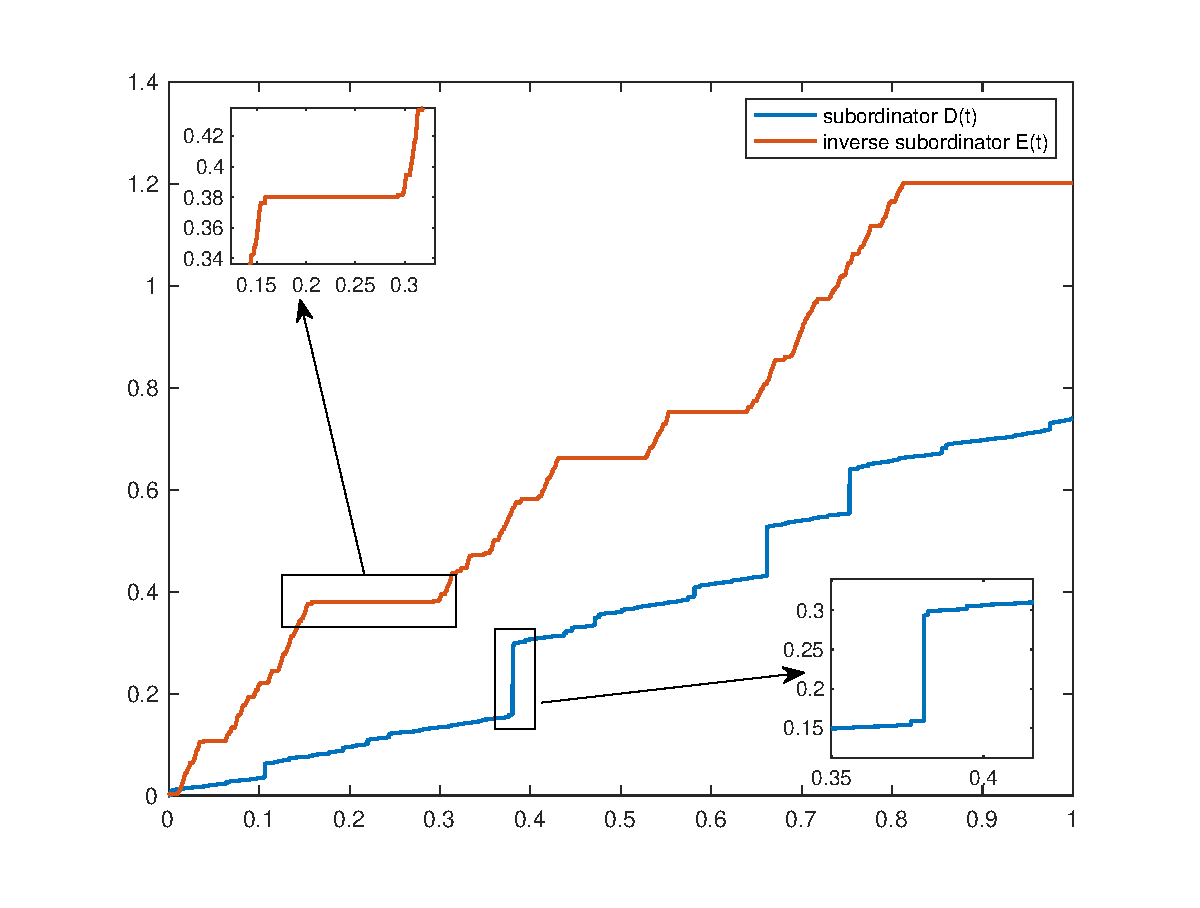
\includegraphics[width=0.45\linewidth]{DE.eps}
	\hfill
	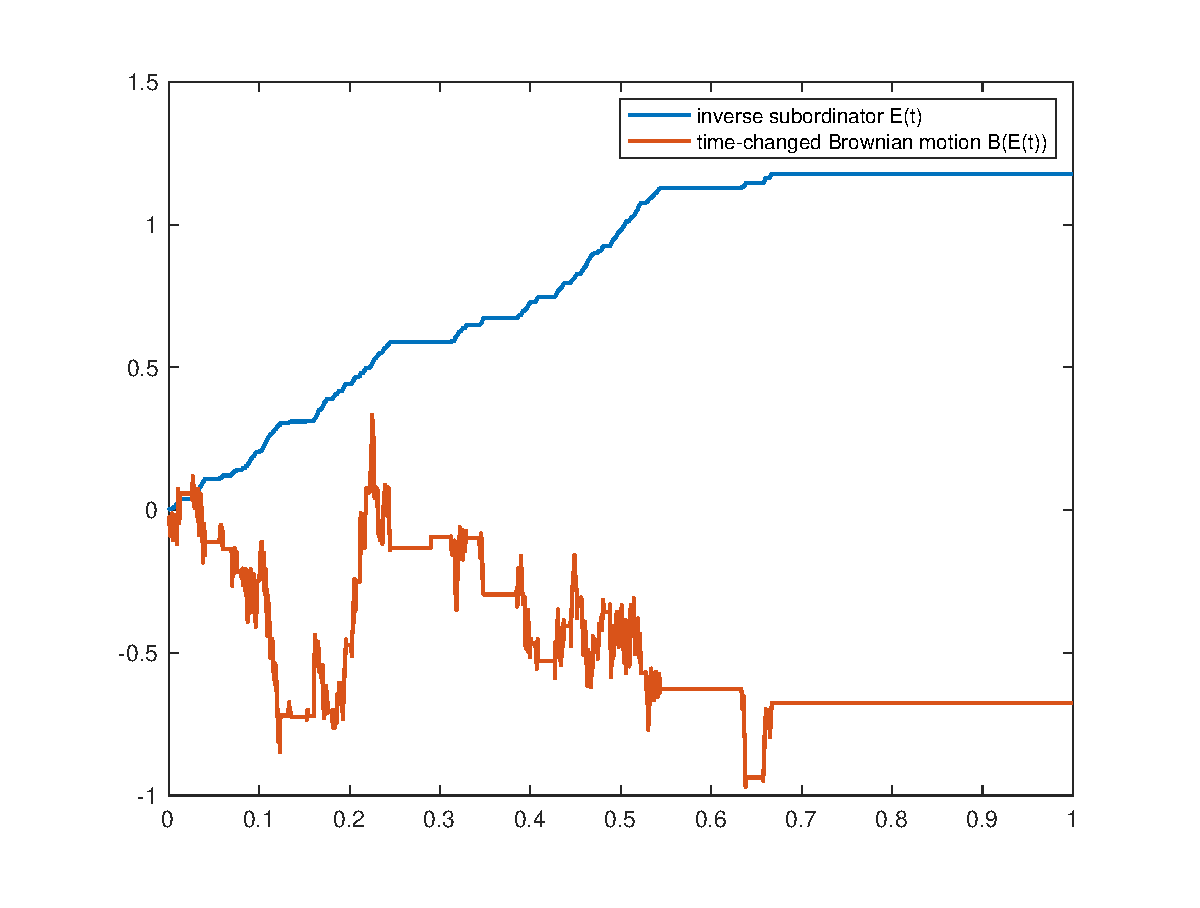
\includegraphics[width=0.45\linewidth]{BE.eps}
	\caption{The left figure shows the subordinated $D$ with stability index $\alpha = 0.8$ and the corresponding inverse subordinator $E$. The right figure shows the inverse subordinator $E$ with stability index $\alpha = 0.8$ and the corresponding time-changed Brownian motion.
	}
	\label{fig:image1}
	\vspace{-2ex}
\end{figure}

\( E \) and \( B \circ E \) both start from 0. For the quadratic variation, we have
$$
[B \circ E, B \circ E] = E \quad \text{and} \quad [E, E] = [B \circ E, E] = 0.
$$
For more details on stochastic calculus for time-changed semimartingales, see Section 4 of \cite{kobayashi2011stochastic}.

Now, let's introduce the Lamperti transformation for time change. 
Let \( S = (l, r) \), where \( -\infty \leq l < r \leq \infty \), and let \( a \) and \( b \) be continuously differentiable functions from \( S \) to \( S \). Consider the following SDE:
\begin{equation}\label{original SDE}
	dy(t) = a(y(t))dE(t) + b(y(t))dB(E(t))
\end{equation}
and assume it has a unique strong solution in \( S \), i.e.,
$$
\mathbb{P}(y(t) \in S, \: t \geq 0) = 1.
$$
If \( b(x) > 0 \) holds for all \( x \in S \), then we can use the Lamperti transformation
\begin{equation}\label{Lamperti}
	F(x) = \lambda \int^x \frac{1}{b(y)} dy
\end{equation}
for some \( \lambda > 0 \). Provided \( F^{-1}: F(S) \to S \) is well-defined, let \( x(t) = F(y(t)) \). Using the time-change Itô formula from \cite{umarov2018beyond}, we get:
\begin{equation}\label{basic SDE}
	dx(t) = f(x(t)) dE(t) + \lambda dB(E(t))
\end{equation}
where
$$
f(x) = \lambda \left( \frac{a(F^{-1}(x))}{b(F^{-1}(x))} - \frac{1}{2} b^{\prime}(F^{-1}(x)) \right), \quad x \in F(S),
$$
and \( F(D) = (F(l), F(r)) \). This transformation converts the nonlinear term of the diffusion into the drift term. In the subsequent part of this paper, we will focus on studying SDE \eqref{basic SDE} with additive noise.

Now, we describe an approximation method for the inverse subordinated process \( E \) given in  \cite{magdziarz2009langevin} and \cite{magdziarz2009stochastic}. Fix an equidistant step size \(\delta > 0\) and a time interval \( T > 0 \). To approximate \( E \) over the interval \([0, T]\), we first simulate the sample path of the subordinated process \( D \) with independent and stationary increments, setting \( D_0 = 0 \), and then proceed with the rule \( D_i^\delta := D_{i-1}^\delta + Z_i \), where \( i = 1, 2, 3, \ldots \), and \( (Z_i)_{i \in \mathbb{N}} \) is an i.i.d. sequence with each \( Z_i \) following the distribution \( Z = \Delta D_\delta \). We stop this process once we find an integer \( N \) such that \( T \in [D_{N\delta}, D_{(N+1)\delta}) \). Note that an \(\mathbb{N}\)-valued random variable \( N \) indeed exists because \( D_t \to \infty \) as \( t \to \infty \) almost surely. To generate the random variables \( (Z_i) \), one can use the algorithm provided in Chapter 6 of [2]. Next, define \( E^\delta := (\min(n \in \mathbb{N}; D_{n\delta} > t) - 1) \delta \). The process \( E^\delta = (E_t^\delta)_{t \geq 0} \) is a non-decreasing step function with constant jump size \(\delta\), and the \( i \)-th waiting time is \( Z_i = D_i^\delta - D_{i-1}^\delta \). Indeed, it is easy to see that for \( n = 0, 1, 2, \ldots, N \), when \( t \in [D_{n\delta}, D_{(n+1)\delta}) \), \( E^\delta = n\delta \). Specifically, \( E^\delta = N\delta \). As stated in [10,16], the process \( E^\delta \) effectively approximates \( E \); that is, almost surely,


\[
E_t - \delta \leq E^\delta \leq E_t \quad \text{for all} \quad t \in [0, T].
\]


Now, for \( n = 0, 1, 2, \ldots, N \), set


\[
\tau_n = D_{n\delta}.
\]



Assuming the independence between \( B \) and \( D \), we can approximate the Brownian motion \( B \) over time steps \(\{0, \delta, 2\delta, \ldots, N\delta\}\). Based on this, define the discrete-time process \(\left(X_{\tau_n}\right)_{n\in\{0,1,2,\ldots, N\}}\) as \( X_0 := x_0 \), and for \( n = 0, 1, 2, \ldots, N-1 \), we have

\begin{equation}\label{stostep}
	X_{\tau_{n+1}} := X_{\tau_n}  + f\left(X_{\tau_n}\right)\left(E_{\tau_{n+1}}-E_{\tau_n}\right)  + \sigma\left(B_{E_{\tau_{n+1}}}-B_{E_{\tau_n}}\right).
\end{equation}

Due to the relationship \( E_{\tau_{n}} = n\delta \), the above equation is equivalent to

\begin{equation}\label{nostostep}
	X_{\tau_{n+1}} :=X_{\tau_n}  + f\left(X_{\tau_n}\right)\delta + \sigma\left(B_{(n+1)\delta}-B_{n\delta}\right).
\end{equation}

Note that although the expression \cref{nostostep} seems to take non-random time steps, in fact, we do take random time steps \(\tau_0, \tau_1, \tau_2, \ldots, \tau_N\) to discretize the driving process \( E = \left(E_t\right)_{t \geq 0} \) and \( B \circ E = \left(B_{E_t}\right)_{t \geq 0} \), as shown in \cref{stostep}; thus, the key characteristic of the random trapping events in the time-change process (i.e., generating constant time intervals) is actually captured by the random step sizes \(\tau_{n+1} - \tau_n = D_{(n+1)\delta} - D_{n\delta} = \Delta D_{\delta}\). Additionally, note that we do not discretize the SDE using non-random time steps; if we did, it would become very difficult because the driving processes \( E \) and \( B \circ E \) do not have independent increments nor stationary increments.

To define a continuous-time process \(\left(X_t^\delta\right)_{t\in[0, T]}\), we use continuous interpolation; that is, when \(s \in \left[\tau_n, \tau_{n+1}\right)\),

\begin{equation}\label{intX}
	X_s:= X_{\tau_n} +  \int_{\tau_n}^s f\left(X_{\tau_n}\right) \, dE_r + \int_{\tau_n}^s \sigma dB_{E_r}.
\end{equation}

Define



\[
n_t = \max\left\{n \in \mathbb{N} \cup \{0\}; \tau_n \leq t\right\} \text{ for } t \geq 0.
\]



Then it is clear that for any \( t > 0 \), we have \( \tau_{n_t} \leq t < \tau_{n_t+1} \). Using \cref{nostostep} and the identity \( X_s - x_0 = \sum_{i=0}^{n_s-1} \left(X_{\tau_{i+1}} - X_{\tau_i}\right) + \left(X_s - X_{\tau_{n_s}}\right) \), we can express \( X_s - x_0 \) as



\[
\sum_{i=0}^{n_s-1} \left[ f\left(E_{\tau_i}, X_{\tau_i}\right)\delta + \sigma\left(B_{(i+1)\delta} - B_{i\delta}\right)\right] + \left(X_s - X_{\tau_{n_s}}\right).
\]



where we used \( i\delta = E_{D_{i\delta}} = E_{\tau_i} \). Using \cref{intX} and the fact that \(\tau_i = \tau_{n_r}\) for any \( r \in [\tau_i, \tau_{i+1}) \), we can rewrite the latter in a more tractable form:

\begin{equation}
	X_s = x_0 + \int_{0}^{s} f\left(X_{\tau_{n_r}}\right) \, dE_r + \int_{0}^{s} \sigma \, dB_{E_r}.
\end{equation}

Introducing the following three lemmas on time change from \cite{umarov2018beyond}:

\begin{lemma}[First Variable Change Formula]\label{first}
	Let B be a one-dimensional standard Brownian motion.
	If $H \in L(B(t), \mathcal{F}_t)$, then $H_{E(t-)} \in L(B_{E(t)}, \mathcal{F}_{E_t})$.
	Furthermore, for all $t \geqslant 0$, almost everywhere
	$$
	\int_0^{E_t} H_s dB(s) = \int_0^t H_{E(s-)} dB_{E(s)}.
	$$
\end{lemma}
\begin{lemma}[Second Variable Change Formula]\label{second}
	Let B be a one-dimensional standard Brownian motion. Assume $D$ and $E$ satisfy $[D \longrightarrow E]$ or $[D \longleftarrow E]$.
	Assume $B$ and $E$ are synchronized. If $K \in L(B_{E(t)}, \mathcal{F}_{E_t})$, then $(K_{D(t-)}) \in L(B(t), \mathcal{F}_{E(D_t)})$.
	Furthermore, for all $t \geqslant 0$, almost everywhere
	$$
	\int_0^t K_s dB_{E(s)} = \int_0^{E_t} K_{D(s-)} dB(s).
	$$
\end{lemma}

\begin{lemma}[Itô Formula]\label{ito}
	Let B be a one-dimensional standard Brownian motion. Let $D$ and $E$ satisfy $[  D\longrightarrow E ]$ or $[  D\longrightarrow E ] .$ X is a stochastic process defined by the following SDE:
	$$X(t):=\int_0^tA(s)ds+\int_0^tF(s)dE(s)+\int_0^tG(s)dB(E(s))$$
	where $A(s)\in L( t, \mathcal{F} _{E(t)})$, $F(s)\in L( E(t), \mathcal{F} _{E(t)})$, and $G(s)\in L( B(E(s)), \mathcal{F} _{E(t)})$. If $f\in C^2( \mathbb{R} )$, then
	$f(X(t))$ is an $\mathcal{F}_{E(t)}$-semimartingale, and for all $t \ge 0$, we have
	$$\begin{aligned}
		&f(X(t))-f(0)=\int_{0}^{t}f^{\prime}(X(s))A(s)ds+\int_{0}^{E(t)}f^{\prime}\left(X(D(s-))\right)F(D(s-))ds\\
		&+\int_{0}^{E(t)}f^{\prime}\big(X(D(s-))\big)G(D(s-))dB(s)+\frac{1}{2}\int_{0}^{E(t)}f^{\prime\prime}\big(X(D(s-))\big)\big\{G(D(s-))\big\}^{2}ds.
	\end{aligned}$$
\end{lemma}

Next, introduce the discrete Gronwall inequality:
\begin{lemma}\label{gronwall}
	Let $\Delta t > 0,g_n,\lambda _n \in \mathbb{R},\eta > 0,a_1=0$, and suppose $1-\eta \Delta E_j > 0$, $1 + \lambda _n > 0,n \in \mathbb{N}$. If
	\begin{equation*}
		a_{n+1} \leq a_n(1+\lambda _n)+\eta a_{n+1}\Delta E_n +g_{n+1}
	\end{equation*}
	then the following inequality holds:
	\begin{equation}
		a_n \leq \sum\limits_{j=0}^{n-1}\prod_{i=j}^{n}(1-\eta\Delta E_i)g_{j+1}\prod\limits_{l=j+1}^{n-1}(1+\lambda _l)
	\end{equation}
\end{lemma}

The following lemma is crucial for proving the main theorems in this paper, quoting the lemma from \cite{nane2016stability}.

\begin{lemma}\label{slowerthant}
	Assume that in the Laplace transform of the inverse subordinated process $E(t)$, $\psi(s)=s^{\alpha}$. Then
	\begin{equation}
		\lim_{t\to\infty}\frac{E_t}{t}=0,\:a.s.
	\end{equation}
\end{lemma}


\begin{lemma}
	If $E$ is the inverse of the subordinated process $D$, and its Laplace exponent $\psi$ has a regular variation index at infinity $\beta \in [0, 1)$. If $\beta = 0$, further assume $\nu(0, \infty) = \infty$. Fix $\lambda > 0$, $t > 0$, and $r > 0$.
	\begin{enumerate}
		\item[(1)] If $r < \frac{1}{1 - \beta}$, then $\mathbb{E}\left[ e^{\lambda E_t^r} \right] < \infty$.
		\item[(2)] If $r > \frac{1}{1 - \beta}$, then $\mathbb{E}\left[ e^{\lambda E_t^r} \right] = \infty$.
	\end{enumerate}
	
\end{lemma}

\begin{lemma}\label{main lemma}
	For any given $0 = t_0 < ih < t_1 < t_2 < \ldots < t_n < (i+1)h$, we have:
	\begin{equation}
		\mathbb{E}\left[\int_{ih}^{(i+1)h}
		\int_{ih}^{t_n} \ldots \int_{ih}^{t_2} 1 dE(t_1) \ldots dE(t_{n-1}) dE(t_n)\right] \le Ch^{1+(n-1)\beta}
	\end{equation}
	where \(C\) is a constant independent of \(h\).
\end{lemma}

\begin{proof}
	Now, introduce the random measure \(\Pi\) on \([0, \infty)\), defined as \(\Pi((s, t]) = E(t) - E(s)\), where \(t > s \geq 0\). Let \(\{C(t)\}_{t \geq 0}\) be a Cox process driven by \(\Pi\), i.e., conditional on \(\Pi = \lambda\), the distribution of \(\{C(t)\}\) is equivalent to that of an inhomogeneous Poisson process with intensity \(\lambda\). Note that according to \cite{kingman1964doubly}, \(\{C(t)\}\) is a renewal process with the renewal function:
	\begin{equation}
		u(t) = \mathbb{E}[C(t)] = \mathbb{E}[E(t)] = \frac{t^\alpha}{\Gamma(\alpha+1)}
	\end{equation}
	For the renewal process \(C(t)\), see \cite{daley2003introduction}, we obtain
	\begin{equation*}
		\mathbb{E}[\mathrm{d}C(t_n)\ldots \mathrm{d}C(t_1)] = \prod_{i=1}^n u^{\prime}(t_i - t_{i-1})\mathrm{d}t_i
	\end{equation*}
	where \(0 = t_0 < t_1 < t_2 < \ldots < t_n\). Since the factorial moments of the Cox process \(C(t)\) are equal to the ordinary moments of its driving measure \(\Pi\), see \cite{daley2003introduction}, we get
	\begin{equation*}
		\mathbb{E}[\mathrm dE(t_n)\ldots \mathrm dE(t_1)] = \prod_{i=1}^n u'(t_i - t_{i-1})\mathrm d t_i.
	\end{equation*}
	Thus:
	\begin{align*}
		I &= \mathbb{E}\left[\int_{ih}^{(i+1)h}
		\int_{ih}^{t_n}\int_{ih}^{t_{n-1}} \ldots \int_{ih}^{t_{2}} 1 dE(t_1) \ldots dE(t_{n-2}) dE(t_{n-1}) dE(t_n)\right] \\
		&= \int_{ih}^{(i+1)h}\int_{ih}^{t_n}\int_{ih}^{t_{n-1}}
		\ldots \int_{ih}^{t_{2}} 1 \mathbb{E}\left[dE(t_1) \ldots dE(t_{n-2}) dE(t_{n-1}) dE(t_n)\right] \\
		&= \frac{\alpha^n}{\Gamma^n(\alpha+1)}
		\int_{ih}^{(i+1)h}\int_{ih}^{t_n}\int_{ih}^{t_{n-1}} \ldots \int_{ih}^{t_{2}} \prod_{i=1}^{i=n} (t_i - t_{i-1})^{\alpha -1} d t_1 \ldots d t_{n-1} d t_n
	\end{align*}
	Next, consider the integral term separately:
	\begin{equation*}
		I_{1}=\int_{ih}^{t_{2}} (t_{2} - t_1)^{\alpha -1} t_1^{\alpha - 1} d t_1
	\end{equation*}
	Make the following transformation: let \( t_{1} = ih + s_{1}h \) and \( t_2 = ih + s_2h \), where \(h\) is the step size, hence \( s_1, s_{2} \in [0,1] \). Since we do not consider time at the origin, \(i = \frac{T}{h}\) where \(T\) is a time range, thus
	\begin{align*}
		I_1 &= \int_{0}^{s_{2}} (s_{2} - s_{1})^{\alpha -1} h^{\alpha -1} (ih + s_1h)^{\alpha - 1} h d s_1 \\
		&= h^{\alpha} \int_{0}^{s_{2}} (s_{2} - s_{1})^{\alpha -1} (ih + s_1h)^{\alpha - 1} d s_1
	\end{align*}
	Since \( (ih + s_1h)^{\alpha - 1} \) is monotonically decreasing with respect to \( s_1 \) in \( [0,1] \), and the integrand and integration range in \( I_n \) are positive, we have
	\begin{align*}
		I_1 &\le h^{\alpha} \int_{0}^{s_{2}} (s_{2} - s_{1})^{\alpha -1} (ih)^{\alpha - 1} d s_1 \\
		&= T^{\alpha - 1} h^{\alpha} \int_{0}^{s_{2}} (s_{2} - s_{1})^{\alpha -1} d s_1
	\end{align*}
	Let \( w_1 = s_{2} - s_{1} \), thus
	\begin{equation*}
		I_1 \le T^{\alpha - 1} h^{\alpha} \int_{0}^{s_{2}} (s_{2} - s_{1})^{\alpha -1} d s_1
		= T^{\alpha - 1} h^{\alpha} \int_{0}^{s_{2}} w_1^{\alpha -1} d w_1
		= \frac{T^{\alpha - 1} s_{2}^\alpha}{\alpha} h^{\alpha}
	\end{equation*}
	Therefore:
	\begin{equation*}
		I \le Ch^\alpha
		\int_{ih}^{(i+1)h}\int_{ih}^{t_n}\int_{ih}^{t_{n-1}} \ldots \int_{ih}^{t_{3}} 
		\prod_{i=3}^{n}(t_i-t_{i-1})^{\alpha -1} d t_{2} \ldots d t_{n-1} d t_n
	\end{equation*}
	Similarly, analyzing the following integral:
	\begin{equation*}
		I_{2} = \int_{ih}^{t_{3}}(t_{3}-t_{2})^{\alpha -1}
		d t_{2} \le Ch^\alpha 
	\end{equation*}
	Therefore:
	\begin{equation*}
		I \le Ch^{2\alpha}
		\int_{ih}^{(i+1)h}\int_{ih}^{t_n}\int_{ih}^{t_{n-1}} \ldots \int_{ih}^{t_{4}} 
		\prod_{i=4}^{n}(t_i-t_{i-1})^{\alpha -1} d t_{3} \ldots d t_{n-1} d t_n
	\end{equation*}
	By iterating this process, we get:
	\begin{equation*}
		I \le Ch^{(n-1)\alpha}\int_{ih}^{(i+1)h} 1 d t_1 \le Ch^{1+(n-1)\alpha}
	\end{equation*}
\end{proof}



\section{Main results: the strong convergence of EM method}

\begin{assumption}\label{Lipschitz}
	In this section, we assume that the drift coefficient \(f\) of the SDE \cref{basic SDE} satisfies the global \textnormal{Lipschitz} condition, that is, there exists a constant \(K > 0\) such that
	\begin{equation}
		|f(x) - f(y)| \le K|x - y|.
	\end{equation}
\end{assumption}

\begin{assumption}\label{linear growth}
	In this section, we assume that the drift coefficient \(f\) of the SDE \cref{basic SDE} satisfies the linear growth condition, that is, there exists a constant \(K > 0\) such that
	\begin{equation}
		|f(x)| \le K(1 + |x|).
	\end{equation}
\end{assumption}

\begin{assumption}\label{momentEM}
	In this section, we assume that the drift coefficient \(f\) of the SDE \cref{basic SDE} is twice continuously differentiable, and there exists a constant \(K > 0\) such that
	\begin{equation}
		|f(x)f'(x)| + |\sigma f'(x)| + |\sigma^2 f''(x)| \leq K(1 + |x|).
	\end{equation}
\end{assumption}

The following proposition aims to derive sufficient conditions for the existence of the \( p \)-th moment of \( \sup_{0 \leq r \leq T} |X_r| \), where \( X \) is the solution to the SDE \cref{basic SDE}. These conditions are necessary for establishing the main theorems of this paper.
\begin{proposition}\label{main pro1}
	Let \( X \) be the solution to the SDE \cref{basic SDE}, where \( f \) satisfies \cref{Lipschitz} and \cref{linear growth}. Then for any \( p \ge 1 \), there exist constants \( c_1, c_2 \) such that \( \mathbb{E}_{B}[Y_T^{(p)}] < c_1 e^{c_2E_T } \), where \( Y_t^{(p)} := 1 + \sup\limits_{0 \le r \le t} |X_r|^p \).
\end{proposition}
\begin{proof}
	Let \( S_{\ell} := \inf\{ t \geq 0 : Y_{t}^{(p)} > \ell \} \) for \( \ell \in \mathbb{N} \). Since the solution \( X \) has continuous paths and \( Y_{t}^{(p)} < \infty \) for each \( t \geq 0 \), \( S_{\ell} \uparrow \infty \) as \( \ell \to \infty \). For \( \mathbb{P}_D \) almost every path, we first apply the Gronwall-type inequality to the function \( t \mapsto \mathbb{E}_B[Y_{t \wedge S_{\ell}}^{(p)}] \) for a fixed \( \ell \), then let \( t = T \) and let \( \ell \to \infty \) in the resulting inequality to establish the upper bound for \( \mathbb{E}_B[Y_T^{(p)}] \). Note that by the definition of \( S_{\ell} \),
	
	
	\[
	\int_{0}^{t} \mathbb{E}_B[Y_{r \wedge S_{\ell}}^{(p)}] \, dE_r \leq \ell E_t < \infty,
	\]
	
	
	which allows us to safely apply the Gronwall-type inequality.
	
	Suppose \( p \geq 2 \), as the result for \( 1 \leq p < 2 \) follows directly by applying the result for \( p \geq 2 \) and Jensen's inequality. By the time-changed Itô formula, we have \( X_s^p = x_0^p + J_s + K_s \), where
	
	
	\[
	J_s := \int_0^s \sigma p X_r^{p-1} \, dB_{E_r};
	\]
	
	
	
	
	\[
	K_s := \int_0^s \left\{ p X_r^{p-1} f(X_r) + \frac{\sigma^2}{2} p (p-1) X_r^{p-2} \right\} \, dE_r.
	\]
	
	
	Fix \( t \in [0, T] \) and \( \ell \in \mathbb{N} \). By \cref{linear growth} and the inequality \( (x + y + z)^p \leq c_p (x^p + y^p + z^p) \), where \( x, y, z \geq 0 \) and \( c_p = 3^{p-1} \), we have
	
	
	\[
	\mathbb{E}_B\left[ \sup_{0 \leq s \leq t \wedge S_{\ell}} |K_s| \right] \leq \left( p c_p K + \frac{1}{2} p(p-1) c_p K^2 \right) \int_0^{t \wedge S_{\ell}} \mathbb{E}_B[Y_r^{(p)}] \, dE_r.
	\]
	
	
	Since \( (J_s)_{s \geq 0} \) is a local martingale, applying the BDG inequality gives
	
	
	\[
	\mathbb{E}_B\left[\sup_{0 \leq s \leq t \wedge S_{\ell}} |J_s| \right] \leq b_1 \mathbb{E}_B \left[\left( \int_0^{t \wedge S_{\ell}} \sigma^2 p^2 X_r^{2p-2} \, dE_r \right)^{1/2}\right],
	\]
	
	
	thus,
	
	
	\[
	\mathbb{E}_B \left[\sup_{0 \leq s \leq t \wedge S_{\ell}} |J_s| \right] \leq b_1 \mathbb{E}_B \left[ p c_p K \left( Y_{t \wedge S_{\ell}}^{(p)} \int_0^{t \wedge S_{\ell}} Y_r^{(p)} \, dE_r \right)^{1/2} \right]
	\]
	
	
	
	
	\[
	\leq \frac{1}{2} \mathbb{E}_B \left[Y_{t \wedge S_{\ell}}^{(p)}\right] + 2b_1^2 p^2 c_p^2 K^2 \int_0^{t \wedge S_{\ell}} \mathbb{E}_B \left[Y_r^{(p)}\right] \, dE_r,
	\]
	
	
	where the last inequality follows from the basic inequality \( (ab)^{1/2} \leq a/\lambda + \lambda b \) for any \( a, b, \lambda > 0 \), with \( \lambda := 2b_1 p c_p K \).
	Note that for any non-negative process \( (L_t)_{t \geq 0} \),
	
	
	\[
	\int_0^{t \wedge S_{\ell}} L_r \, dE_r \leq \int_0^t L_{r \wedge S_{\ell}} \, dE_r.
	\]
	
	
	Indeed, the inequality is obvious if \( t \leq S_{\ell} \), while if \( t > S_{\ell} \),
	
	
	\[
	\int_0^{S_{\ell}} L_r \, dE_r + \int_{S_{\ell}}^t L_{S_{\ell}} \, dE_r \geq \int_0^{t \wedge S_{\ell}} L_r \, dE_r.
	\]
	
	
	Thus, from the above estimates for \( J_s \) and \( K_s \), we have
	
	
	\[
	\mathbb{E}_B[Y_{t \wedge S_{\ell}}^{(p)}] \leq 2(1 + |x_0|^p) + 2K^2\left(p c_p K + \left(p(p-1) c_p / 2 + 2b_1^2 p^2 c_p^2\right) \right) \int_0^t \mathbb{E}_B[Y_{r \wedge S_{\ell}}^{(p)}] \, dE_r.
	\]
	
	
	Applying the Gronwall-type inequality, we get
	
	
	\[
	\mathbb{E}_B[Y_{t \wedge S_{\ell}}^{(p)}] \leq 2(1 + |x_0|^p) e^{2K^2E_T \left(p c_p K + \left(p(p-1) c_p / 2 + 2b_1^2 p^2 c_p^2\right) \right) }.
	\]
	
	
	Letting \( t = T \) and letting \( \ell \to \infty \), since \( \xi(u) \) is independent of \( \ell \), and by applying the monotone convergence theorem, we obtain
	
	\begin{equation}\label{boundY}
		\mathbb{E}_B[Y_T^{(p)}] \leq 2(1 + |x_0|^p) e^{2K^2E_T \left(p c_p K + \left(p(p-1) c_p / 2 + 2b_1^2 p^2 c_p^2\right) \right)}.
	\end{equation}
	% By taking expectation \(\mathbb{E}_D\) on both sides, we get \(\mathbb{E}[Y_T^{(p)}] \leq \mathbb{E}[ce^{cE_T}] < \infty\), which is due to the result of Theorem 1 in \cite{jin2019strong}. 
\end{proof}

Next, we prove the first important theorem.
\begin{theorem}\label{main th EM1}
	Let $X$ be the solution to the SDE \textnormal{\cref{basic SDE}}, under the conditions of \textnormal{\cref{Lipschitz}}, \textnormal{\cref{linear growth}}, and \textnormal{\cref{momentEM}}.
	Let $X_t$ be the EM numerical method defined in \textnormal{\cref{nostostep}} and \textnormal{\cref{intX}}. Then there exists a constant $C > 0$ independent of $\delta$, such that for all $\delta \in (0,1)$,
	
	
	\[
	\mathbb{E} \left[ \sup_{0 \leq s \leq T} | X(s) - X_t | \right] \leq C \delta.
	\]
	
	
	Hence, $X_t$ converges strongly to $X(t)$ uniformly with order 1 on $[0, T]$.
\end{theorem}

\begin{proof}
using the Itô formula expansion, we obtain
\begin{align}\label{afterito}
	X_{\tau_{n+1}} &= X_{\tau_n} +  \int_{\tau_n}^{\tau_{n+1}} f(X_{\tau_n}) \, \mathrm{d}E_r + \int_{\tau_n}^{\tau_{n+1}} \sigma \, \mathrm{d}B_{E_r} + R_{(\tau_n, \tau_{n+1})}; \\
	R_{(a,b)} &:=  \int_a^b \int_a^{s} \left( f(X_{\tau_{n_{r}}})f'(X_{\tau_{n_{r}}}) + \frac{\sigma ^2}{2} f''(X_{\tau_{n_{r}}})  \right) \, \mathrm{d}E_{r} \, \mathrm{d}E_{s} + \int_a^b \int_a^{s} \sigma f'(X_{\tau_{n_{r}}})   \, \mathrm{d}B_{E_{r}} \,\mathrm{d}E_{s},
\end{align}
Subtracting \cref{afterito} from \cref{intX}, we get
$$Z_t := \sup_{0 \leq s \leq t} | X_s - {X_s^\delta} | \leq I_1 + I_2,$$ where

$$
\begin{aligned}
	&I_1 := \sup_{0 \leq s \leq t} \left| \int_0^s f(X_{\tau_{n_r}}) - f(X_{\tau_{n_r}}^\delta)  \, \mathrm{d}E_r \right|; \\
	&I_2 := \sup_{0 \leq s \leq t} \left| \sum_{i=0}^{n_s - 1} R_{(\tau_{t}, \tau_{t+1})} + R_{(\tau_{n_s}, s)} \right|.
\end{aligned}
$$

For $I_1$, from \cref{Lipschitz}, we get
\begin{equation}\label{I1}
	\mathbb{E}_B[I_1] \leq K \int_0^t \mathbb{E}_B[Z_r] \, \mathrm{d}E_r.
\end{equation}

The main technical part involves the remainder term $I_2$, which consists of two different double integrals: $\mathrm{d}E_{r_1} \, \mathrm{d}E_{r_2}$ and $\mathrm{d}B_{E_{r_1}} \, \mathrm{d}E_{r_2}$. We will handle these integrals separately below.

For the first integral $\mathrm{d}E_{r_1} \, \mathrm{d}E_{r_2}$,
\begin{align}
	& \quad \mathbb{E}_B \left[\sup_{0 \leq s \leq t} \left| \int_0^s \int_{\tau_{n_2}}^{r_2} ff'  + \frac{\sigma^2}{2} f'' \, \mathrm{d}E_{r_1} \, \mathrm{d}E_{r_2} \right|\right] \nonumber \\
	&\leq  \frac{3}{2}K \mathbb{E}_B[Y_T^{(1)}] \int_0^t \int_{\tau_{n_{r_2}}}^{r_2} \, \mathrm{d}E_{r_1} \, \mathrm{d}E_{r_2} \nonumber \\
	&\leq  \frac{3}{2}K E_T \mathbb{E}_B[Y_T^{(1)}] \delta.  \label{I21}
\end{align}
The appearance of $\delta$ instead of $\delta^{\alpha}$ is primarily due to our use of a randomly discretized numerical scheme.

On the other hand, we need to estimate $\mathbb{E}_B \left[\sup_{0 \leq s \leq t} |M_{n_s} + U_s|\right]$, where $M_0 := 0$, and for $n \geq 1$, $M_n := \sum_{i=0}^{n-1} L_i$,
$$
L_i := \int_{\tau_i}^{\tau_{i+1}} \int_{\tau_i}^{r_2} \sigma f' \, \mathrm{d}B_{E_{r_1}} \, \mathrm{d}E_{r_2}, \quad U_s := \int_{\tau_{n_s}}^s \int_{\tau_{n_s}}^{r_2} \sigma f' \, \mathrm{d}B_{E_{r_1}} \, \mathrm{d}E_{r_2}.
$$

This expression, along with the proofs of Lemmas 5.7.1 and 10.8.1 in reference [12], shows that the discrete-time process $(M_n)_{n \geq 0}$ is a square-integrable $((\mathcal{F}_{n\delta})_{n \geq 0}, \mathbb{P}_B)$-martingale with initial value 0. Thus, by the BDG inequality (3.2) and the independence of $L_i$,

$$
\mathbb{E}_B \left[\sup_{0 \leq s \leq t} M_{n_s}^2\right] \leq b_2 \sum_{i=0}^{n_t-1} \mathbb{E}_B [L_i^2].
$$
Therefore, by the Cauchy-Schwarz inequality,
\begin{align}
	\mathbb{E}_B\left[\sup_{0\leq s\leq t}M_{n_s}^2\right] 
	&\leq b_2\delta\sum_{i=0}^{n_t-1}\int_{\tau_i}^{\tau_{i+1}}\mathbb{E}_B
	\left[\int_{\tau_i}^{r_2}\left|\sigma f'\right|^2\mathrm{d}E_{r_1}\right]
	\mathrm{d}E_{r_2} \nonumber \\
	&\leq2b_2\delta K^2\mathbb{E}_B[Y_T^{(2)}]\sum_{i=0}^{n_t-1}\int_{\tau_i}^
	{\tau_{i+1}}(E_{r_2}-E_{\tau_i})\mathrm{d}E_{r_2} \nonumber \\
	&\leq 2b_2E_TK^2\mathbb{E}_B[Y_T^{(2)}]\delta^2. \label{I221}
\end{align}
On the other hand, 
\begin{align}
	\mathbb{E}_B\left[\sup_{0\leq s\leq t}U_s^2\right]  
	&\leq\mathbb{E}_B\biggl[\sup_{0\leq s\leq t}(E_s-E_{\tau_{n_s}})\int_{\tau_{n_s}}^s\left|\int_{\tau_{n_s}}^{r_2}\sigma f'\mathrm{d}B_{E_{r_1}}\right|^2\mathrm{d}E_{r_2}\biggr] \nonumber \\ &\leq\delta\int_0^t\mathbb{E}_B\left[\sup_{s\in[r_2,t]}\left|\int_{\tau_{n_s}}^{r_2}\sigma f'\mathrm{d}B_{E_{r_1}}\right|^2\right]\mathrm{d}E_{r_2}.\label{I222}
\end{align}
Since $\{(\tau_{n_s},r_2)~:~r_2~\leq~s~\leq~t\}~\subset~\{(\tau_{n_{r_2}},u)~:~\tau_{n_{r_2}}~\leq~u~\leq~r_2\},$
\begin{align*}
	&\quad\mathbb{E}_B\Big[\sup_{S\in[r_2,t]}\Big|\int_{\tau_x}^{r_2}\sigma f'\mathrm{d}B_{E_{r_1}}\Big|^2\Big]  \\
	&\le \mathbb{E}_B\left[\sup_{u\in[\tau_{n_{r_2}},r_2]}\left|\int_{\tau_{n_{r_2}}}^u\sigma f'\mathrm{d}B_{E_{r_1}}\right|^2\right] \\
	&\leq b_2\mathbb{E}_B\left[\int_{\tau_{n_{r_2}}}^{r_2}\left|\sigma f'\right|^2\mathrm{d}E_{r_1}\right]\\
	&\leq 2b_2K^2\mathbb{E}_B[Y_T^{(2)}]\delta.
\end{align*}
Therefore, the upper bound for \cref{I222} is $2b_2E_TK^2\mathbb{E}_B[Y_T^{(2)}]\delta^2.$ Combining this with \cref{I221}:
\begin{equation}\label{I22}
	\mathbb{E}_B\left[\sup_{0\leq s\leq t}|M_{n_s}+U_s|^2\right] 
	\leq 8b_2E_TK^2\mathbb{E}_B[Y_T^{(2)}]\delta^2. 
\end{equation}
From the estimates \cref{I21} and \cref{I22},
\begin{equation}\label{I2}
	\mathbb{E}_B[I_2] 
	\leq \left\{\frac{3}{2}E_T\mathbb{E}_B[Y_T^{(1)}]+(8b_2E_T\mathbb{E}_B[Y_T^{(2)}])^{1/2}\right\}K\delta. 
\end{equation}

Now, combining \cref{I1} and \cref{I2} with $\mathbb{E}_B[Y_T^{(1)}]\leq\sqrt{2}\mathbb{E}_B[Y_T^{(2)}]^{1/2}$:
\begin{equation*}
	\mathbb{E}_B[Z_t] 
	\leq \xi_2(E_T)\mathbb{E}_B[Y_T^{(2)}]^{1/2}\delta + K\int_0^t\mathbb{E}_B[Z_r] \mathrm{d}E_r.
\end{equation*}

where $\xi_2(u) := K(\frac{3\sqrt{2}}{2}u + (8b_2u)^{1/2}).$
Applying the Gronwall-type inequality, taking $\mathbb{E}_D$ on both sides and using the Cauchy-Schwarz inequality:
\begin{equation*}
	\mathbb{E}[Z_T] \leq \mathbb{E}[\xi_2^4(E_T)]^{1/4}\mathbb{E}[(Y_T^{(2)})^2]^{1/4}\mathbb{E}[e^{2KE_T}]^{1/2}\delta.
\end{equation*}
Since $\mathbb{E}[e^{\lambda E_t}] < \infty$ and $\mathbb{E}[E^n(t)] < \infty$ for any $\lambda>0, t>0,n>0$, and combining this with \cref{main pro1}, the theorem holds.

\end{proof}

\section{Main results: the strong convergence of BEM method}

\begin{assumption}\label{super linear growth}
	In this section, we assume that the drift coefficient \(f\) of the SDE \cref{basic SDE} satisfies the super-linear growth condition, that is, there exists a constant \(K > 0\) and \(\gamma > 1\) such that
	\begin{equation}
		|f(x)| \le K(1+|x|^{\gamma}).
	\end{equation}
\end{assumption}

\begin{assumption}\label{momentBEM}
	In this section, we assume that the drift coefficient \(f\) of the SDE \cref{basic SDE} is twice continuously differentiable, and there exists a constant \(K > 0\) and \(\gamma > 1\) such that
	\begin{equation}
		|f(x)f'(x)| + |\sigma f'(x)| + |\sigma^2 f''(x)| \leq K(1 + |x|^{\gamma}).
	\end{equation}
\end{assumption}

\begin{assumption}\label{Local Lipschitz}
	In this section, we assume that the drift coefficient $f$ of the SDE \cref{basic SDE} satisfies the one-sided Lipschitz condition, that is, there exists a constant $K > 0$ such that
	\begin{equation}
		(x-y)(f(x)-f(y)) \le K|x-y|^2.
	\end{equation}
\end{assumption}

For the existence and uniqueness proof of the solution to the SDE \cref{basic SDE} under the condition of the drift coefficient \(f\) being monotone, refer to the proof in \cite{umarov2018beyond} for the case where the drift satisfies the global Lipschitz condition. Similar to \textnormal{\cref{nostostep}} and \textnormal{\cref{intX}}, we can derive the corresponding BEM numerical scheme.
\begin{equation}\label{nostostepY}
	X_{\tau_{n+1}} :=X_{\tau_n} + f\left(X_{\tau_{n+1}}\right)\delta + \sigma\left(B_{(n+1)\delta}-B_{n\delta}\right).
\end{equation}

\begin{equation}\label{intY}
	X_s:= X_{\tau_n} + \int_{\tau_n}^s f\left(X_{\tau_{n+1}}\right) \, dE_r + \int_{\tau_n}^s \sigma dB_{E_r}.
\end{equation}

Similar to \cref{main pro1}, we can derive the following proposition.
\begin{proposition}\label{main pro2}
	Let $X$ be the solution to the SDE \cref{basic SDE}, where $f$ satisfies \cref{monotony} and \cref{super linear growth}. Then for any $p \ge 1$, there exist constants $c_1, c_2$ such that $\mathbb{E}_{B}[Y_T^{(p)}] < c_1 e^{c_2E_T }$, where $Y_t^{(p)} := 1 + \sup\limits_{0 \le r \le t} |X_r|^p$.
\end{proposition}

Next, we prove the second important theorem.
\begin{theorem}\label{main th BEM1}
	Let $X$ be the solution to the SDE \textnormal{\cref{basic SDE}}, under the conditions of \textnormal{\cref{super linear growth}}, \textnormal{\cref{momentBEM}}, and \textnormal{\cref{Local Lipschitz}}. 
	Let $X_t$ be the BEM numerical method defined in \textnormal{\cref{nostostepY}} and \textnormal{\cref{intY}}. Then there exists a constant $C > 0$ independent of $\delta$, such that for all $\delta \in (0,1)$,
	
	
	\[
	\mathbb{E} \left[ \sup_{0 \leq s \leq T} | X(s) - X_t | \right] \leq C \delta.
	\]
	
	
	Hence, $X_t$ converges strongly to $X(t)$ uniformly with order 1 on $[0, T]$.
\end{theorem}




\section{Numerical simulations}


\begin{example}[Time-Changed OU Process]
	Consider the time-changed Ornstein-Uhlenbeck process driven by Brownian motion
	\begin{equation}\label{linear}
		dX(t) = \mu X(t) dE_t + \sigma dB_{E_t}.
	\end{equation}
\end{example}
For \cref{Lipschitz}, \cref{linear growth}, and \cref{momentEM}, it is clear that this example satisfies these conditions. The corresponding EM numerical scheme for this equation is:
\begin{align*}
	X_{i+1} = (1 + \mu \Delta E_i) X_i + \sigma \Delta B_{E_i}.
\end{align*}

In our numerical experiments, we focus on the $L_1$ error at the endpoint $T = 1$, so we define
\begin{align*}
	e_T^{i} = \mathbb{E}\left|X_T^{\delta _4} - X_T^{\delta _i}\right|,
\end{align*}
where $X_T^{\delta _i}$ is the simulated value at $T$ with step size $\delta _i$, $\delta _i = 2^{-i}$. For our numerical experiments, we set $\mu = 1$ and $\sigma = 1$, and use the Monte Carlo method:
\begin{align*}
	e_{T}^i \approx \frac{1}{10^3}\sum_{j=1}^{10^3}\left|X_T^{\delta _{14}} - X_T^{\delta _i}\right|, \quad \text{where } i = 6, 7, 8, 9.
\end{align*}
We use the step size $2^{-14}$ as a reference and estimate the $L_1$ error using step sizes ${2^{-6}, 2^{-7}, 2^{-8}, 2^{-9}}$. The table below compares the convergence rates and errors for different $\alpha$ values.
\begin{table}[h]
	\centering
	\begin{tabular}{>{\centering\arraybackslash}m{3cm}|>{\centering\arraybackslash}m{1cm}>{\centering\arraybackslash}m{1cm}>{\centering\arraybackslash}m{1cm}>{\centering\arraybackslash}m{1cm}>{\centering\arraybackslash}m{1cm}>{\centering\arraybackslash}m{1cm}>{\centering\arraybackslash}m{1cm}>{\centering\arraybackslash}m{1cm}}
		\hline
		$\alpha$  & 0.3000 & 0.4000 & 0.5000 & 0.6000 & 0.7000 & 0.8000 & 0.9000 & 1.0000 \\ \hline
		Convergence Order & 0.9937 & 1.0345 & 1.0195 & 1.0204 & 1.0261 & 1.0318 & 1.0283 & 1.0281 \\ 
		\hline
	\end{tabular}
	\caption{Convergence rates and errors for different $\alpha$ values}
	\label{tab:example5columns}
\end{table}


\begin{figure}[htp!]
	\centering
	\includegraphics[width=0.45\linewidth]{stochastic_EM_0.4.eps}
	\hfill
	\includegraphics[width=0.45\linewidth]{stochastic_EM_0.8.eps}
	\caption{$L_1$ error of the EM method with stochastic steps. The left figure shows $\alpha = 0.4$ and the right figure shows $\alpha = 0.8$.}
	\label{fig:stochastic_EM}
	\vspace{-2ex}
\end{figure}

\begin{example}
	Consider the time-changed CIR process driven by Brownian motion
	\begin{equation}\label{CIR}
		dy(t)=\kappa(\theta-y(t))dE(t)+\sigma\sqrt{y(t)}dB(E(t)),\quad t\geq0,\quad y(0)>0.
	\end{equation}
\end{example}
If $2\kappa\theta\geq\sigma^{2}$, then $D=(0,\infty)$ and \cref{unique} holds in $(\alpha, \beta) = (0,\infty)$. 
Moreover, using the Itô formula with $X(t) = F(y(t))$, where $F$ is defined by \cref{Lamperti}, we can obtain the Lamperti transformation of the time-changed CIR process:
\begin{equation}
	dX(t)=f(X(t))dE(t)+\frac12\sigma dB(E(t)),\quad t\geq0,\quad X(0)=\sqrt{y(0)}.
\end{equation}
where
\begin{equation}
	f(X)=\dfrac{1}{2}\kappa\left(\theta_vX^{-1}-X\right),\quad X>0
\end{equation}
with $\theta_v=\theta-\frac{\sigma^2}{4\kappa}$. The BEM numerical scheme is as follows:
\begin{equation}
	X_{t_{i+1}}=X_{t_{i}}+f(X_{t_{i+1}})\Delta E_i+\frac{1}{2}\sigma\Delta B_{E_i},\quad k=0,1,\dots 
\end{equation}
We observe that
\begin{equation}
	f'(X)=-\frac{1}{2}\kappa(\theta_vX^{-2}+1)
\end{equation}
and
\begin{equation}
	f(X)f'(X)+\frac{\sigma^2}{2}f''(X)=-\frac{\kappa^2}{4}(\theta_v^2X^{-3}-X)+\frac{1}{2}\kappa\theta_vX^{-3}\sigma^2.
\end{equation}
Therefore, to satisfy \cref{moment}, it is sufficient to have
\begin{equation}
	\sup_{0\leq t\leq T}\mathbb{E}[X(t)^{-3}]=\sup_{0\leq t\leq T}\mathbb{E}[y(t)^{-\frac{3}{2}}] < \infty.
\end{equation}
For the bounded moments of the time-changed CIR process $y(t)$, we have
\begin{equation}
	\sup\limits_{0\leq t\leq T}\mathbb{E}[y(t)^q]<\infty\quad\text{for}\quad q>-\frac{2k\theta}{\sigma^2}.
\end{equation}
Next, we verify the bounded moments for the exact solution of the time-changed CIR process \cref{CIR}.
\begin{proposition}
	For the time-changed CIR process driven by Brownian motion \cref{CIR} with $y_0>0$ and $1<p<\frac{2K\theta}{\sigma^2}-1$, there exists a constant $C$ such that
	\begin{equation*}
		\sup\limits_{t\in[0,T]}\mathbb{E}\left[\left(y(t)\right)^{-p}\right]\leq C(1+y(0)^{-p}).
	\end{equation*}
\end{proposition}
\begin{proof}
	Define the stopping time $\tau_{n}=\mathrm{inf}\{0<s\leq T;y(s)\leq1/n\}$. By applying the Itô formula, we obtain
	$$\begin{aligned}
		\mathbb{E}_B\left[(y(t\wedge\tau_{n}))^{-p}\right] &= y(0)^{-p} - p\mathbb{E}_B\left[\int_{0}^{t\wedge\tau_{n}}\frac{K(\theta-y(s))}{(y(s))^{p+1}}dE(s)\right]\\
		&+ p(p+1)\frac{\sigma^{2}}{2}\mathbb{E}_B\left[\int_{0}^{t\wedge\tau_{n}}\frac{1}{(y(s))^{p+1}}dE(s)\right] \\
		&\leq y(0)^{-p} + pK\int_{0}^{t}\mathbb{E}_B\left(\frac{1}{(y(s\wedge\tau_{n}))^{p}}\right)dE(s) \\
		&+\mathbb{E}_B\left[\int_0^{t\wedge\tau_n}\frac{p\left(\frac{(p+1)\sigma^2}{2}-K\theta\right)}{(y(s))^{p+1}}dE(s)\right].
	\end{aligned}$$
	We can find a positive constant $\underline C$ such that when $\frac{(p+1)\sigma^2}{2}-K\theta<0$, for any $y(0)=x>0$, we have
	$$\frac{p\left(\frac{(p+1)\sigma^2}{2}-K\theta\right)}{x^{p+1}}\leq \underline C.$$
	Therefore,
	$$\mathbb{E}_B\left[(y(t\wedge\tau_n))^{-p}\right]\leq y(0)^{-p}+\underline{C}E(T)+pK\int_0^t\sup_{r\in[0,s]}\mathbb{E}_B\left[(y(r\wedge\tau_n))^{-p}\right]dE(s).$$
	Using the Gronwall inequality, we obtain
	$$\sup\limits_{t\in[0,T]}\mathbb{E}_B\left[(y(t\wedge\tau_n)^x)^{-p}\right]\leq\left(y(0)^{-p}+\underline{C}E(T)\right)\exp(pKE(T)).$$
	Taking $\mathbb{E}_D$ on both sides and using the Cauchy-Schwarz inequality, we get
	$$\begin{aligned}
		\sup\limits_{t\in[0,T]}\mathbb{E}\left[(y(t\wedge\tau_n)^x)^{-p}\right]&\leq\mathbb{E}\left[\left(y(0)^{-p}+\underline{C}E(T)\right)\exp(pKE(T))\right]\\
		&\leq\sqrt{\mathbb{E}\left[\left(y(0)^{-p}+\underline{C}E(T)\right)^2\right]\mathbb{E}\left[\exp(2pKE(T))\right]}.
	\end{aligned}$$
	From \cite{jum2014strong}, we have
	\begin{equation}
		\mathbb{E}[E^n(t)]=\frac{n!}{\Gamma(n\alpha+1)}t^{n\alpha},
	\end{equation}
	\begin{equation}
		\mathbb{E}[e^{\lambda E(t)}]<\infty,
	\end{equation}
	where $\lambda \in \mathbb{R}, t > 0$. Finally, letting $n \to +\infty$, we complete the proof.
\end{proof}

\begin{remark}
	Here, we have only proved the existence of moments for $1 < p < \frac{2K\theta}{\sigma^2} - 1$. Actually, it can be proven that $p < \frac{2K\theta}{\sigma^2}$, but the proof is too complicated and not necessary for our results.
\end{remark}
For \cref{moment}, it can be verified that it is sufficient to ensure that $1 < \frac{4}{3}\frac{\kappa\theta}{\sigma^2}$ holds. This interval is covered by $1 < p < \frac{2K\theta}{\sigma^2} - 1$, so it suffices to ensure that $p$ is within this range. As for \cref{monotony}, it can be easily verified that there exists such a $\kappa$ in $(0, \infty)$ to satisfy this condition. Therefore, from \cref{main th}, it follows that for the time-changed CIR process, the strong convergence order of the BEM numerical scheme is $\alpha$.


\begin{example}
	Consider the time-changed CEV process driven by Brownian motion
	\begin{equation}\label{CEV}
		dy(t)=\kappa(\theta-y(t))dE(t)+\sigma y(t)^\alpha dB_{E(t)}.
	\end{equation}
\end{example}

Here, $0.5 < \alpha < 1, \kappa, \theta, \sigma > 0$. By transforming $X(t)=F(y(t))$ where $F$ is defined in \cref{Lamperti}, we get that \cref{monotony} holds in $(\alpha, \beta) = (0, \infty)$, and we have
$$dX(t)=f(X(t))dE(t)+(1-\alpha)\sigma dB(E(t)),$$
where
$$f(X)=(1-\alpha)\left(\kappa\theta X^{-\frac{\alpha}{1-\alpha}}-\kappa X-\frac{\alpha\sigma^2}{2}X^{-1}\right),\quad X>0.$$

We also need to verify \cref{moment}. Since $\alpha > 0.5$, we have $\frac{1}{1-\alpha} > 2$, so
$$f^{\prime}(X)=-\alpha\kappa\theta X^{-\frac{1}{1-\alpha}}-(1-\alpha)\kappa+(1-\alpha)\frac{\alpha\sigma^2}{2}X^{-2},\quad X>0,$$
and
$$f^{\prime\prime}(X)=\frac{\alpha}{1-\alpha}\kappa\theta X^{-\frac{2-\alpha}{1-\alpha}}-(1-\alpha)\alpha\sigma^2X^{-3}.$$

The following proposition verifies the bounded moments for the exact solution of the time-changed CEV process \cref{CEV}.

\begin{proposition}
	For the time-changed CEV process \cref{CEV} driven by Brownian motion, with $X_0>0$, for any $\frac{1}{2} < \alpha < 1$ and any $p > 0$, there exists a constant $C$ such that
	\begin{equation*}
		\sup\limits_{t\in[0, T]} \mathbb{E}\left[\left(y(t)\right)^{-p}\right] \leq C(1 + y(0)^{-p}).
	\end{equation*}
\end{proposition}
\begin{proof}
	Define the stopping time $\tau_{n}=\inf\{0 < s \leq T; y(s) \leq 1/n\}$. Using the Itô formula, we get
	$$\begin{aligned}
		\mathbb{E}_B\left[(y(t\wedge\tau_{n}))^{-p}\right] &= y(0)^{-p} - p \mathbb{E}_B\left[\int_{0}^{t\wedge\tau_{n}} \frac{\kappa(\theta-y(s))}{(y(s))^{p+1}} dE(s)\right] \\
		&+ p(p+1) \frac{\sigma^{2}}{2} \mathbb{E}_B\left[\int_{0}^{t\wedge\tau_{n}} \frac{1}{(y(s))^{p+2(1-\alpha)}} dE(s)\right] \\
		&\leq y(0)^{-p} + p\kappa \int_{0}^{t} \mathbb{E}_B\left(\frac{1}{(y(s\wedge\tau_{n}))^{p}}\right)dE(s) \\
		&+ \mathbb{E}_B\left[\int_0^{t\wedge\tau_n}\left(p(p+1)\frac{\sigma^2}{2}\frac{1}{(y(s))^{p+2(1-\alpha)}}-p\frac{\kappa\theta}{(y(s))^{p+1}}\right)dE(s)\right]
	\end{aligned}$$
	We can find a positive constant $C$ such that, for any $y(0)=x > 0$,
	$$\left(p(p+1)\frac{\sigma^2}{2}\frac{1}{x^{p+2(1-\alpha)}}-p\frac{\kappa\theta}{x^{p+1}}\right) \leq C.$$
	From the calculations, we get that $\underline C = p(2\alpha-1)\frac{\sigma^2}{2}\left[(p+2(1-\alpha))\frac{\sigma^2}{2\kappa\theta}\right]^{\frac{p+2(1-\alpha)}{2\alpha-1}}$ is the smallest upper bound. Therefore,
	$$\mathbb{E}_B\left[(y(t\wedge\tau_n))^{-p}\right] \leq y(0)^{-p} + \underline{C}E(T) + p\kappa \int_0^t \sup_{r\in[0, s]} \mathbb{E}_B\left[(y(r\wedge\tau_n))^{-p}\right] dE(s).$$
	Applying the Gronwall inequality, we get
	$$\sup\limits_{t\in[0, T]} \mathbb{E}_B\left[(y(t\wedge\tau_n)^x)^{-p}\right] \leq \left(y(0)^{-p} + \underline{C}E(T)\right) \exp(p\kappa E(T)).$$
	Taking the expectation $\mathbb{E}_D$ on both sides and using the Cauchy-Schwarz inequality, we get
	$$\begin{aligned}
		\sup\limits_{t\in[0, T]} \mathbb{E}\left[(y(t\wedge\tau_n)^x)^{-p}\right] &\leq \mathbb{E}\left[\left(y(0)^{-p} + \underline{C}E(T)\right) \exp(p\kappa E(T))\right] \\
		&\leq \sqrt{\mathbb{E}\left[\left(y(0)^{-p} + \underline{C}E(T)\right)^2\right]\mathbb{E}\left[\exp(2p\kappa E(T))\right]}
	\end{aligned}$$
	From \cite{jum2014strong}, we have
	\begin{equation}
		\mathbb{E}[E^n(t)] = \frac{n!}{\Gamma(n\alpha+1)}t^{n\alpha}
	\end{equation}
	\begin{equation}
		\mathbb{E}[e^{\lambda E(t)}] < \infty
	\end{equation}
	where $\lambda \in \mathbb{R}, t>0$. Finally, letting $n \to +\infty$, we complete the proof.
\end{proof}

From the Lamperti transformation, we know that the inverse moments of $X(t)$ can be controlled by the inverse moments of $y(t)$, so \cref{moment} is satisfied. Therefore, according to \cref{main th}, we conclude that the convergence order of the BEM numerical scheme for the time-changed CEV process driven by Brownian motion is $\alpha$.

\begin{figure}[htp!]
	\centering
	\includegraphics[width=0.45\linewidth]{BEMalpha=0.3.eps}
	\hfill
	\includegraphics[width=0.45\linewidth]{BEMalpha=0.8.eps}
	\caption{Absolute error estimation between the numerical solution and the analytical solution of the time-changed CIR process. The left figure shows $\alpha=0.3$, and the right figure shows $\alpha=0.8$.}
	\label{fig:image}
	\vspace{-2ex}
\end{figure}

%% Appendix
%\appendix
%\section{An example appendix}
%
%The contents of the appendix are here.
%
%\begin{lemma}
%Test Lemma.
%\end{lemma}
%
%This is an equation in the appendix.
%\begin{equation}\label{eq:abc}
%  a^2+b^2=c^2.
%\end{equation}


\section*{Acknowledgments}

We would like to acknowledge the assistance of volunteers in putting together this example manuscript and supplement.


% References
\bibliographystyle{plain}
%\bibliographystyle{abbrv}

\bibliography{reference}


\end{document}

